% ====================================================================
% v4-01.tex — Chapter 2 (v4: 통계열역학 챕터, 분포 명시 전개)
%   출발 skeleton: base_ch2_v3.tex (265줄, Bernardi 가역열 survey).
%   v4 목표: 코인 하프셀(전극 vs Li) 데이터 해석용 엔트로피·가역 발열
%            통계열역학 챕터. 분배함수 → 점유 분포 → config/vib/electronic
%            엔트로피 명시 전개. 섞임/겹침 수식(A/B/C/D/I) 포함.
%   범위: 코인 하프셀 단독. 전셀 합성 범위 외.
%   build: xelatex 2-pass (kotex).
% ====================================================================
\documentclass[11pt,a4paper]{article}
\usepackage[margin=22mm]{geometry}
\usepackage{kotex}
\setmonofont{D2Coding}[Scale=MatchLowercase]
\usepackage{amsmath,amssymb,mathtools,bm}
\usepackage{booktabs,longtable,array}
\usepackage{enumitem}
\usepackage{amsthm}
\usepackage{hyperref}
\usepackage{fancyhdr}
\usepackage{lastpage}
\usepackage{setspace}
\usepackage{pgf,tikz}
\usetikzlibrary{arrows.meta,calc}
\setstretch{1.12}
\setlength{\parskip}{0.45em}\setlength{\parindent}{0pt}\setlength{\headheight}{14pt}
\setlength{\emergencystretch}{3em}
\hypersetup{colorlinks=true, linkcolor=blue, urlcolor=blue, citecolor=blue,
  pdftitle={흑연 음극 dQ/dV --- Chapter 2 (v4): 통계열역학 엔트로피·가역 발열}}
\pagestyle{fancy}\fancyhf{}
\lhead{흑연 음극 $dQ/dV$ --- Ch.\,2 (v4, 통계열역학)}\rhead{\thepage/\pageref{LastPage}}
\renewcommand{\headrulewidth}{0.4pt}
\newtheorem*{keybox}{핵심}
\newtheorem*{srcbox}{문헌 근거}
\newtheorem*{warnbox}{주의}
\newcommand{\dd}{\mathrm{d}}
\newcommand{\rxn}{\mathrm{rxn}}
\newcommand{\eq}{\mathrm{eq}}
\newcommand{\rev}{\mathrm{rev}}
\newcommand{\irr}{\mathrm{irr}}
\newcommand{\oc}{\mathrm{oc}}
\newcommand{\config}{\mathrm{config}}
\newcommand{\vib}{\mathrm{vib}}
\newcommand{\el}{\mathrm{el}}
\newcommand{\eff}{\mathrm{eff}}
\renewcommand{\theequation}{2.\arabic{equation}}
\renewcommand{\thesection}{2.\arabic{section}}
\title{\textbf{\LARGE Chapter 2}\\[0.35em]
  \Large 흑연 음극 코인 하프셀의 엔트로피와 가역 발열\\[0.2em]
  \large --- 분배함수 $\to$ 점유 분포 $\to$ 배위·진동·전자 엔트로피 $\to$ $\dot{Q}_{\rev}$\\[0.15em]
  \normalsize (v4, 통계열역학 챕터)}
\author{}\date{}

\begin{document}
\maketitle
\tableofcontents
\clearpage

% ====================================================================
\section*{서 --- 왜 엔트로피엔 통계가 필요한가}
\addcontentsline{toc}{section}{서 --- 왜 통계가 필요한가}
\label{sec:intro}
% ====================================================================

Chapter~1은 흑연 음극의 $dQ/dV$ 한 곡선을 전이별 평형 중심 전위
$U_j(T)=(-\Delta H_{\rxn,j}+T\,\Delta S_{\rxn,j})/F$와 동역학 꼬리로 설명했다.
그 식 안에는 이미 \emph{엔트로피} $\Delta S_{\rxn,j}$가 살아 있다.
그런데 이 양이 \emph{왜} 온도마다 달라지고,
왜 $x$(탈리튬화율)에 따라 $+29$에서 $-16$\,J\,mol$^{-1}$K$^{-1}$으로 크게 변하는지는
Ch1만으로는 설명되지 않는다.
엔트로피는 미시 상태의 흩어짐 척도이므로, 그 \emph{원천}은 리튬 이온이 어떤 분포로 격자 자리를
채우느냐에 있다.

코인 하프셀에서 전극 전위 $U_{\oc}(x,T)$를 여러 온도에서 측정하면,
기울기 $\partial U_{\oc}/\partial T$---엔트로피 계수(entropy coefficient)---를 얻는다.
이것이 가역 발열(reversible heat)의 원천이다:
\begin{equation}
  \boxed{\;\dot{Q}_{\rev}=-I\,T\,\frac{\partial U_{\oc}}{\partial T}
    =-\frac{IT}{F}\,\Delta S(x)\;.}
  \label{eq:qrev_def}
\end{equation}
이 \emph{사슬} 전체를 단계적으로 유도하는 것이 본 장의 목표다.
가역 발열은 \emph{분포를 재배열하는 열}이므로,
$\partial U_{\oc}/\partial T(x)$를 이해하려면 리튬 점유 분포를 명시해야 한다.

\begin{keybox}
본 장의 세 분포 기반 엔트로피:
(1)~배위(configurational) --- 격자기체 점유 분포,
(2)~진동(vibrational) --- 포논 Bose--Einstein 분포,
(3)~전자(electronic) --- Fermi--Dirac 분포.
이 셋이 측정 $\partial U_{\oc}/\partial T(x)$를 구성한다.
\end{keybox}

\medskip\noindent
\textbf{코인 하프셀 단독.}\;
본 장의 $U_{\oc}$, $\Delta S$, $\dot{Q}_{\rev}$는 모두 \emph{코인 하프셀(전극 vs.\ Li)}
단일 전극 기준이다. 전셀 합성($\partial U_{\mathrm{cell}}/\partial T
=\partial U_{\mathrm{cat}}/\partial T - \partial U_{\mathrm{an}}/\partial T$)은
본 장 범위 밖이며 혼동하지 않는다.

% ====================================================================
\section{가역열과 비가역열 --- Bernardi 에너지 수지}\label{sec:bernardi}
% ====================================================================

전지 발열의 출발점은 Bernardi, Pawlikowski, Newman의 일반 에너지 수지다~\cite{bernardi1985}.
부반응·혼합·상변화를 무시한 단일 활물질 한계에서:
\begin{equation}
  \dot{Q}=I\,(U_{\oc}-V)-I\,T\,\frac{\partial U_{\oc}}{\partial T}\,,
  \label{eq:bernardi}
\end{equation}
($I>0$ 방전, $V$ 단자 전압, $U_{\oc}$ 개방회로 평형 전위).
우변 첫째 항 $I(U_{\oc}-V)\ge0$은 과전압 소산---비가역열 $\dot{Q}_{\irr}$.
둘째 항이 \emph{가역열} $\dot{Q}_{\rev}$이며 부호가 양방향이다.

전기화학 열역학의 표준 항등식
$\Delta G=-FU_{\oc}$, $\Delta S=-\partial(\Delta G)/\partial T$에서 즉시
\begin{equation}
  \Delta S=F\,\frac{\partial U_{\oc}}{\partial T}\;,
  \label{eq:thermo_id}
\end{equation}
이 나오므로 $\dot{Q}_{\rev}=-(IT/F)\,\Delta S(x)$ --- 이것이 식~\eqref{eq:qrev_def}이다
\cite{newman,msmr_partI}.

\begin{srcbox}
부호 규약: 본 장은 $U_{\oc}$ 기준 $\Delta S=+F\,\partial U_{\oc}/\partial T$로 통일한다.
일부 문헌의 $-$ 부호는 셀 전압 정의 차이에서 온다.
$I>0$(방전)에서 $\partial U_{\oc}/\partial T>0$이면 $\dot{Q}_{\rev}<0$(흡열).
\end{srcbox}

% ====================================================================
\section{격자기체 분배함수와 점유 분포}\label{sec:partition}
% ====================================================================

\subsection{단일 자리 grand-canonical 앙상블}\label{ssec:single}

흑연 격자를 1몰의 동등 자리($N_A$개) 집합으로 본다.
각 자리는 비거나($\varepsilon=0$) 리튬이 채우거나($\varepsilon=\varepsilon_0$)의
\emph{2-상태 시스템}이다. 화학퍼텐셜 $\mu$를 가진 리튬 저장조(Li 금속)와 열접촉한
grand-canonical 앙상블에서 단일 자리 분배함수는
\begin{equation}
  Z_1 = 1 + e^{-\beta(\varepsilon_0-\mu)}\,,\qquad \beta\equiv\frac{1}{k_BT}\,.
  \label{eq:Z1}
\end{equation}
평균 점유 확률은
\begin{equation}
  \langle n\rangle = \frac{e^{-\beta(\varepsilon_0-\mu)}}{Z_1}
    = \frac{1}{1+e^{\beta(\varepsilon_0-\mu)}}\,.
  \label{eq:FD_form}
\end{equation}
이 식은 Fermi--Dirac 분포와 구조가 동형이다(자리당 2-상태, 스핀 없음).

\paragraph{Ch1 logistic의 기원.}
전기화학 리튬 자리에서 $\varepsilon_0-\mu = -F(V-U_j)$이므로
(전극 전위 $V$, 전이 중심 $U_j$),
$\beta(\varepsilon_0-\mu)=(V-U_j)/(RT/F)$. 따라서
\begin{equation}
  \langle n\rangle=\xi_{\eq,j}
    =\frac{1}{1+\exp\!\bigl[-(V-U_j)/w_j\bigr]}\,,
    \qquad w_j\equiv\frac{RT}{F}\,,
  \label{eq:logistic}
\end{equation}
이것이 Ch1의 logistic 함수 $\xi_{\eq,j}$이다.
\textbf{Ch1의 logistic은 격자기체 단일 자리 점유 확률---통계역학에서 유일하게 도출된다.}
$w=RT/F$는 분포의 에너지 폭이고, 온도 $T$와 함께 넓어진다.

\begin{figure}[h]
\centering
% TikZ: occupancy distribution <n> vs (V-Uj)/w
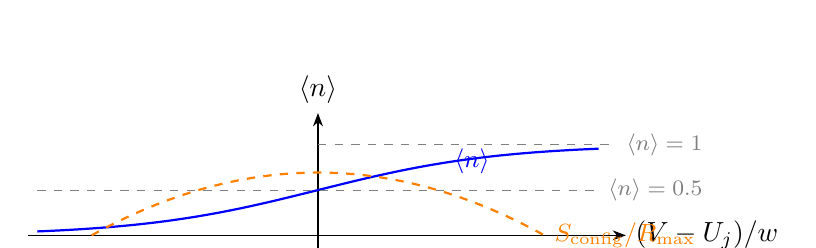
\begin{tikzpicture}[scale=1.15,>=Stealth]
  % axes
  \draw[->] (-3.2,0)--(3.4,0) node[right] {$(V-U_j)/w$};
  \draw[->] (0,-0.15)--(0,1.35) node[above] {$\langle n\rangle$};
  % Fermi curve
  \draw[blue,thick,domain=-3.1:3.1,samples=100]
    plot (\x,{1/(1+exp(-\x))});
  % S_config normalized: use Gaussian approximation centered at 0 (safe)
  % S_config(xi=1/(1+exp(-u))) ~ ln2*(1 - u^2/4) for |u|<2, else 0
  % clamp to safe range u in [-2.5, 2.5]
  \draw[orange,thick,dashed,domain=-2.5:2.5,samples=80]
    plot (\x, {max(0, 0.693*(1-\x*\x/6.25))})
    node[right,font=\small] {$S_\config/R_{\max}$};
  % reference lines
  \draw[gray,dashed] (-3.1,0.5)--(3.1,0.5)
    node[right,font=\footnotesize] {$\langle n\rangle=0.5$};
  \draw[gray,dashed] (0,1)--(3.3,1)
    node[right,font=\footnotesize] {$\langle n\rangle=1$};
  % labels
  \node[blue,font=\small] at (1.7,0.82) {$\langle n\rangle$};
\end{tikzpicture}
\caption{격자기체 단일 자리 점유 분포 $\langle n\rangle=(V-U_j)/w$ (파란 실선, Ch1 logistic)와
  배위 엔트로피 $S_\config=-R[\theta\ln\theta+(1-\theta)\ln(1-\theta)]$ (주황 점선, 정규화).
  $\langle n\rangle=0.5$($V=U_j$)에서 $S_\config$ 최대, 양 끝에서 $\to0$.}
\label{fig:FD_Sconfig}
\end{figure}

\subsection{다자리 Bragg--Williams 평균장}\label{ssec:BW}

자리 간 리튬--리튬 상호작용 에너지 $\Omega$를 평균장(mean-field)으로 도입하면,
1몰 자리의 Gibbs 에너지는
\begin{equation}
  g(\theta)=g_0+RT[\theta\ln\theta+(1-\theta)\ln(1-\theta)]+\Omega\,\theta(1-\theta)\,,
  \label{eq:BW}
\end{equation}
($\theta$: 몰 분율 점유율). Bragg--Williams(BW) 정규 용액이다~\cite{huggins2009,bazant2013}.
$\Omega>0$ 인력, $\Omega<0$ 반발. $\Omega\ge2RT$이면 $g(\theta)$ 쌍봉(bimodal) $\to$ 상분리.
Ch1의 서로 겹치지 않는 개별 전이를 비상호작용($\Omega\to0$) 한계로 볼 수 있다.

% ====================================================================
\section{분포에서 배위 엔트로피로}\label{sec:config}
% ====================================================================

\subsection{Boltzmann--Shannon 엔트로피}\label{ssec:boltzmann}

점유 확률 $p_1=\theta$ (Li-자리), $p_0=1-\theta$ (빈 자리)의 Shannon 엔트로피:
\begin{equation}
  \boxed{\;S_\config = -R\sum_i p_i\ln p_i
    = -R\bigl[\theta\ln\theta+(1-\theta)\ln(1-\theta)\bigr]\;}\quad
    (\text{1몰 자리당})\,.
  \label{eq:Sconfig}
\end{equation}
$\theta=\frac{1}{2}$에서 최대 $R\ln2=5.76$\,J\,mol$^{-1}$K$^{-1}$,
$\theta\to0,1$에서 $\to0$ (순서 정렬, 엔트로피 소멸).
이것이 Ch1 logistic 분포에 대응하는 배위 엔트로피의 닫힌 식이다.

\subsection{부분몰 배위 엔트로피}\label{ssec:partial_molar}

Li 1몰 추가($\theta\to\theta+d\theta$)에 따른 엔트로피 변화---부분몰 배위 엔트로피:
\begin{equation}
  \bar{S}_\config \equiv \frac{\partial S_\config}{\partial\theta}
    = -R\ln\frac{\theta}{1-\theta}\,.
  \label{eq:partial_S}
\end{equation}
희박($\theta\to0$): $\bar{S}_\config\to+\infty$ (리튬이 무질서로 분산).
만충($\theta\to1$): $\bar{S}_\config\to-\infty$ (남은 빈 자리 부족, 정렬 강제).
이것이 $\partial U_{\oc}/\partial T$의 $x$-의존(봉우리 내부) 항이다.

\paragraph{Ch1 로직과의 연결---이중계산 B.}

Ch1 logistic의 전위식은
\begin{equation}
  V(\xi_j)=U_j+\frac{RT}{F}\ln\frac{\xi_j}{1-\xi_j}\,.
  \label{eq:V_logistic}
\end{equation}
온도로 미분하면($\xi_j$ 고정):
\begin{equation}
  \frac{\partial V}{\partial T}\bigg|_{\xi_j}
    =\frac{\Delta S_{\rxn,j}}{F}+\frac{R}{F}\ln\frac{\xi_j}{1-\xi_j}\,.
  \label{eq:dVdT_logistic}
\end{equation}
\textbf{이중계산 B --- 반드시 준수:}
$\Delta S_{\rxn,j}$는 $\xi_j=\frac{1}{2}$($V=U_j$, config 항 $=0$)에서의 \emph{중심 표준값}이다.
Ch1 코드의 피팅 파라미터 $\Delta S_{\rxn,j}$ 자체가 이미 이 규약으로 정의된다.
식~\eqref{eq:dVdT_logistic} 우변 둘째 항 $\frac{R}{F}\ln[\xi_j/(1-\xi_j)]$이
배위(config) $x$-의존이며, $\Delta S_{\rxn,j}$에 \emph{추가로 더하는} 항이다.
이 둘을 중복 가산하면 이중계산이 된다~(\S\ref{sec:mixing_B} 참조).

\begin{warnbox}
$\Delta S_{\rxn,j}$ = 전이 중심 표준값 (vib + electronic 중심, config = 0).\\
배위 $x$-의존 = 분포 폭 $w=RT/F$가 자동으로 생성.\\
둘을 \emph{독립 항}으로 취급해 별개 가산해야 한다 --- 이중계산 금지.
\end{warnbox}

% ====================================================================
\section{진동 엔트로피 (포논 Bose--Einstein 분포)}\label{sec:vib}
% ====================================================================

격자 진동(포논)은 Bose--Einstein 분포를 따른다:
\begin{equation}
  n_k=\frac{1}{e^{\beta\hbar\omega_k}-1}\,,
  \label{eq:BE}
\end{equation}
($\omega_k$: 포논 진동수 모드 $k$). 1몰 격자의 진동 엔트로피는
\begin{equation}
  S_\vib = R\sum_k\bigl[(1+n_k)\ln(1+n_k)-n_k\ln n_k\bigr]\,.
  \label{eq:Svib}
\end{equation}
리튬 삽입 시 C--C 결합과 층간 간격이 변하므로,
삽입 전후 $\Delta S_\vib=S_\vib^\mathrm{after}-S_\vib^\mathrm{before}$.
Reynier 등~\cite{reynier2003}이 보고한 고-$x$ 음의 baseline
($\Delta S<0$ at $x>0.5$)은 주로 이 진동 기여에서 온다:
삽입으로 층간 거리가 줄고 포논 에너지가 높아지면 $n_k$ 감소 $\to$ $S_\vib$ 감소.

실용 근사로서, $\Delta S_\vib$는 Ch1의 피팅 파라미터 $\Delta S_{\rxn,j}$ 중심값에
이미 흡수(전이별 상수 근사)된다. 단, LCO 양극처럼 $x$에 따라 격자 대변형이 급변하는 경우
별도 $x$-의존 진동 항이 필요하다.

% ====================================================================
\section{전자 엔트로피 (Fermi--Dirac 분포)}\label{sec:electronic}
% ====================================================================

전도 전자는 Fermi--Dirac 분포를 따른다:
\begin{equation}
  f(\varepsilon)=\frac{1}{e^{(\varepsilon-E_F)/k_BT}+1}\,.
  \label{eq:FD_el}
\end{equation}
Sommerfeld 전개로 낮은 온도에서 전자 엔트로피는
\begin{equation}
  S_\el = \frac{\pi^2}{3}k_B^2 T\,g(E_F)\cdot N_A\,,
  \label{eq:Sel_sommerfeld}
\end{equation}
($g(E_F)$: Fermi 준위에서 전자 상태 밀도).
부분몰 전자 엔트로피:
\begin{equation}
  \Delta S_\el = \frac{\partial S_\el}{\partial x}<0
  \quad(\text{삽입 기준, Ch1 v9 일관})\,.
  \label{eq:dSel}
\end{equation}
리튬 삽입으로 $E_F$가 이동하고 $g(E_F)$가 바뀌므로 $\Delta S_\el<0$이다.

\paragraph{흑연 vs. LCO.}
흑연 음극은 금속성이 강해 $g(E_F)$가 크지 않고,
Sommerfeld 항은 $T\sim300$\,K에서 배위·진동에 비해 소수 기여다.
LCO 양극은 $x\approx0.5$ 근방 금속--절연체 전이(MIT, metal--insulator transition)에서
$g(E_F)$가 급변하므로 전자 엔트로피가 뚜렷한 $x$-의존성을 가진다
--- Ch2가 이 항을 \emph{FD 분포} 관점에서 가역열 사슬에 통합한다.

% ====================================================================
\section{세 분포 기반 총 엔트로피}\label{sec:total}
% ====================================================================

단일 전이 $j$의 부분몰 전체 반응 엔트로피는
\begin{equation}
  \Delta S(x)\big|_j = \underbrace{\Delta S^0_j}_{\text{중심 표준(vib+el 포함)}}
    + \underbrace{R\ln\!\frac{\xi_j}{1-\xi_j}}_{\text{배위(config 분포)}}
    + \underbrace{\Delta S_\el(x)}_{\text{FD 전자(MIT 구간)}}\,,
  \label{eq:total_entropy}
\end{equation}
(부호 규약: $\xi=$ 탈리튬화 진행률, $\xi\to1$이 희박 Li, $\xi\to0$이 만충).\;
배위 항 부호: 희박($\xi\to1$) $\to$ $R\ln[1/0^+]=+\infty$;
만충($\xi\to0$) $\to$ $R\ln[0^+/1]=-\infty$.

$\partial U_{\oc}/\partial T$ 측정값은 이 세 기여의 합이다:
\begin{equation}
  \boxed{\;\frac{\partial U_{\oc}}{\partial T}(x)
    =\frac{\Delta S(x)}{F}
    =\frac{\Delta S^0_j}{F}+\frac{R}{F}\ln\frac{\xi_j}{1-\xi_j}
      +\frac{\Delta S_\el}{F}\;}\,.
  \label{eq:dUdT_total}
\end{equation}
코인 하프셀의 다온도 측정이 곧 세 분포의 합을 추출하는 실험이다.

% ====================================================================
\section{섞임·겹침 수식}\label{sec:mixing}
% ====================================================================

실제 흑연 $dQ/dV$는 여러 전이가 겹친다.
본 절은 그 겹침을 닫힌 수식으로 처리한다.

\subsection{A. 봉우리 겹침 --- dQ/dV 가중 평균}\label{sec:mixing_A}

관측 평형 전위 $U_{\oc}(x,T)$는 음함수로 정의된다:
\begin{equation}
  \sum_j Q_j\,\xi_{\eq,j}(U_{\oc},T)=Q\,x\,.
  \label{eq:implicit}
\end{equation}
양변을 $T$로 미분(implicit differentiation, $x$ 고정):
\begin{equation}
  \sum_j Q_j\left(\frac{\partial\xi_j}{\partial U}\bigg|_T\,
    \frac{\partial U_{\oc}}{\partial T}\bigg|_x
    +\frac{\partial\xi_j}{\partial T}\bigg|_U\right)=0\,.
  \label{eq:implicit_diff}
\end{equation}
각 기여를 정리하자.
$g_j\equiv\partial\xi_j/\partial V|_T=\xi_j(1-\xi_j)/w_j$ (logistic 도함수, dQ/dV 봉우리 모양).
선두 차수에서 $\partial\xi_j/\partial T|_U\approx-g_j\,\Delta S_{\rxn,j}/F$
(전이 중심의 $T$ 의존 기여, Ch1 $U_j(T)$ 미분). 식~\eqref{eq:implicit_diff}에 대입하면
\begin{equation}
  \boxed{\;\frac{\partial U_{\oc}}{\partial T}(x)
    =\frac{1}{F}\frac{\sum_j Q_j\,g_j(x)\,\Delta S_{\rxn,j}}{\sum_j Q_j\,g_j(x)}\;}\,,
  \label{eq:weighted_mean}
\end{equation}
전이별 $\Delta S_{\rxn,j}/F$를 국소 dQ/dV 비중 $Q_jg_j/\sum Q_jg_j$로 가중한 평균.

겹침 구간에서는 $g_j,g_{j+1}$ 모두 0이 아니므로
$\partial U_{\oc}/\partial T$는 $\Delta S_{\rxn,j}/F$에서 $\Delta S_{\rxn,j+1}/F$로
\emph{연속 이동}한다---계단이 아닌 부드러운 블렌드.

\paragraph{수치 검증 (완전식).}
$\partial\xi_j/\partial T|_U$의 배위 항까지 포함한 \emph{완전식}:
\begin{equation}
  \frac{\partial U_{\oc}}{\partial T}(x)
    =\frac{\sum_j Q_j\,g_j\bigl(\Delta S_j/F+z_j\,R/F\bigr)}{\sum_j Q_j\,g_j}\,,
    \quad z_j=\frac{U_{\oc}(x)-U_j}{w_j}\,,
  \label{eq:full_deriv}
\end{equation}
은 GRAPHITE\_STAGING\_LIT 4-전이 파라미터에서 유한차분(FD, $\Delta T=6$\,K)과
부동소수점 수준($|\mathrm{err}|=0.000\,\mathrm{mV/K}$)으로 일치함을 계산 서브세션이 검증했다
\cite{numericalverif2026}.
식~\eqref{eq:weighted_mean}(단순식)는 배위 항을 의도적으로 분리한 \emph{중심값}이며
최대 $0.184\,\mathrm{mV/K}$ 체계적 차이를 보인다---이것이 배위 항이다.

\begin{figure}[h]
\centering
\begin{tikzpicture}[scale=1.05,>=Stealth]
  % axes: x in [0,6], y in [-0.7,2.0]
  \draw[->](0,0)--(6.4,0) node[right,font=\small]{$x$ (탈리튬화, $\xi\!\to\!1$ 희박)};
  \draw[->](0,-0.7)--(0,2.0) node[above,font=\small]{$\partial U_{\oc}/\partial T$};
  % zero line
  \draw[gray,dashed](0,0)--(6.2,0);
  % Schematic: pure Gaussian peaks only (no logistic, avoids dimension-too-large)
  % peak1: x~0.5, height 1.5 (dS>0, stage 4->3)
  % trough: x~2.5, depth -0.2 (dS~0)
  % peak3: x~3.5, depth -0.3 (dS<0)
  % trough4: x~5.0, depth -1.0 (dS<0, stage 2->1)
  \draw[blue,thick,domain=0.05:6.1,samples=200]
    plot(\x,{ 1.50*exp(-2.0*(\x-0.5)*(\x-0.5))
             +0.00*exp(-3.0*(\x-2.0)*(\x-2.0))
             -0.30*exp(-2.5*(\x-3.5)*(\x-3.5))
             -1.00*exp(-1.5*(\x-5.2)*(\x-5.2))});
  % y-axis ticks
  \draw(0.05,1.5)--(-0.05,1.5) node[left,font=\tiny]{$+0.3$};
  \draw(0.05,-1.0)--(-0.05,-1.0) node[left,font=\tiny]{$-0.17$};
  % annotations
  \node[font=\small] at (1.5,1.7) {$+\Delta S$ (희박)};
  \node[font=\small] at (5.0,-1.25) {$-\Delta S$ (만충)};
\end{tikzpicture}
\caption{흑연 코인 하프셀 $\partial U_{\oc}/\partial T(x)$ 모식도 (schematic).
저-$x$(희박 Li, stage $4\to3$) 구간 양의 봉우리와
고-$x$(만충, stage $2\to1$) 구간 음의 영역.
겹침 구간에서 dQ/dV 가중 평균으로 연속 변화.}
\label{fig:dUdT_schematic}
\end{figure}

\subsection{B. 이중계산 금지 --- 중심 표준값과 배위의 분리}\label{sec:mixing_B}

식~\eqref{eq:full_deriv}에서 배위 항 $z_j R/F$가 명시됐다.
$\Delta S_{\rxn,j}$는 \emph{반드시} $\xi_j=\frac{1}{2}$($z_j=0$, $V=U_j$)에서 정의된 중심 표준값이어야 한다.
만약 $\Delta S_{\rxn,j}$를 임의의 $x$에서 측정한 값(배위 항 포함)으로 설정하고
식~\eqref{eq:full_deriv}의 $z_jR/F$ 항도 더한다면, 배위 기여를 이중 계산하게 된다.

\begin{keybox}
이중계산 B 분리 규칙:\\
$\Delta S_{\rxn,j}$ = 전이 중심($\xi_j=\frac{1}{2}$) 표준값. 여기에 vib + electronic 중심 포함.\\
배위 $x$-의존 = 식~\eqref{eq:full_deriv}의 $z_jR/F$ 항.\\
둘을 \emph{별개}로 더한다. $\Delta S_{\rxn,j}$에 이미 $x$-의존 배위를 넣지 않는다.
\end{keybox}

\subsection{C. 상호작용 $\Omega$와 유효 폭 $w_{\eff}$}\label{sec:mixing_C}

Bragg--Williams 정규 용액~\eqref{eq:BW}에서 평형 등온선의 기울기:
\begin{equation}
  \frac{\dd V_{\eq}}{\dd\xi}=\frac{RT}{F}\!\left[\frac{1}{\xi(1-\xi)}-\frac{2\Omega}{RT}\right].
  \label{eq:isotherm_slope}
\end{equation}
$\xi=\frac{1}{2}$(중심)에서 $(4RT-2\Omega)/F$.
$\Omega\to0$: $4RT/F$ (이상 격자기체). $\Omega>0$: 봉우리 좁아짐. $\Omega\to2RT$: 평탄(상분리 임계).

유효 폭을 중심 기울기 정합으로 정의하면
\begin{equation}
  \boxed{\;w_{\eff}=\frac{w}{1-\Omega/(2RT)}\,,\quad w=RT/F\quad(\Omega<2RT)\;}\,.
  \label{eq:weff}
\end{equation}
$\Omega\to2RT^-$에서 $w_{\eff}\to\infty$---등온선 평탄화, $\partial U/\partial T$ 평탄·불연속.
같은 $x$ 폭에서 봉우리가 좁아지면($\Omega>0$) 단위 $\xi$ 당 $\ln[\xi/(1-\xi)]$가 더 가팔라져
배위 기여가 \emph{증폭}된다.

온도 의존성 주의: $\Omega(T)$가 약하게 변하면 $\partial w_{\eff}/\partial T$가
$\partial U/\partial T$에 2차 기여를 준다(소수, 설계 정밀화 시 고려).

\begin{figure}[h]
\centering
% Schematic: BW isotherms drawn with Bezier/coordinates (no ln, no overflow)
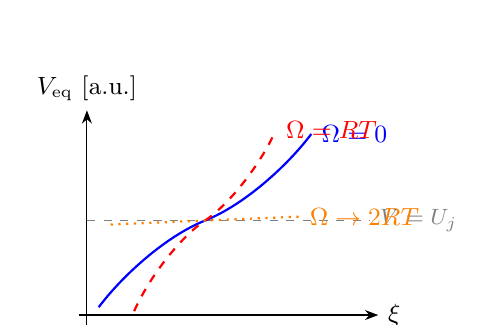
\begin{tikzpicture}[scale=1.0,>=Stealth]
  \draw[->](0,-0.15)--(0,2.6) node[above,font=\small]{$V_{\eq}$ [a.u.]};
  \draw[->](-0.1,0)--(3.7,0) node[right,font=\small]{$\xi$};
  \draw[gray,dashed](0,1.2)--(3.6,1.2)
    node[right,font=\footnotesize]{$V=U_j$};
  % Omega=0: wide S-curve via Bezier (range xi in [0.05,0.95])
  \draw[blue,thick]
    (0.15,0.10) .. controls (0.45,0.50) and (1.0,1.0) ..
    (1.50,1.20) .. controls (2.0,1.40) and (2.55,1.90) ..
    (2.85,2.30) node[right,font=\small]{$\Omega=0$};
  % Omega=RT: narrower S-curve
  \draw[red,thick,dashed]
    (0.60,0.05) .. controls (0.80,0.50) and (1.2,1.0) ..
    (1.50,1.20) .. controls (1.80,1.40) and (2.20,1.90) ..
    (2.40,2.35) node[right,font=\small]{$\Omega=RT$};
  % Omega->2RT: nearly flat (plateau)
  \draw[orange,thick,dotted]
    (0.30,1.15) -- (2.70,1.25)
    node[right,font=\small]{$\Omega\to2RT$};
\end{tikzpicture}
\caption{Bragg--Williams 등온선 $V_{\eq}(\xi)$ 모식도.
$\Omega=0$ (파란 실선)에서 $\Omega=RT$ (빨간 점선)으로 봉우리가 좁아지고,
$\Omega\to2RT$ (주황 점선)에서 평탄화(상분리 임계).
유효 폭 $w_{\eff}=w/(1-\Omega/2RT)$가 발산한다.}
\label{fig:weff}
\end{figure}

\subsection{D. 히스테리시스 --- 분기별 $\partial U/\partial T$와 가역/비가역 분리}\label{sec:mixing_D}

흑연 OCV는 충방전 사이 경로의존(준안정 stacking, stage II 무질서)이다~\cite{hysteresis2018}.
분기 $d$($d=\mathrm{ch}$: 충전, $d=\mathrm{dis}$: 방전)에서 전이 중심이 히스테리시스 갭만큼 이동:
$U_j^{(d)}=U_j\pm\frac{1}{2}\Delta U_j^{\mathrm{hys}}$.

분기별 엔트로피 계수:
\begin{equation}
  \frac{\partial U_{\oc}^{(d)}}{\partial T}(x)
    =\frac{1}{F}\frac{\sum_j Q_j\,g_j^{(d)}(x)\,\Delta S_{\rxn,j}}
      {\sum_j Q_j\,g_j^{(d)}(x)}\,,
  \label{eq:hys_branches}
\end{equation}
($g_j^{(d)}$: 분기 봉우리 모양).

가역·비가역 분리:
\begin{align}
  \frac{\partial U^{\rev}}{\partial T}
    &=\frac{1}{2}\!\left(\frac{\partial U^{\mathrm{ch}}}{\partial T}
      +\frac{\partial U^{\mathrm{dis}}}{\partial T}\right)
    \quad\leftarrow\text{가역 발열의 열역학적 }\Delta S\,,
  \label{eq:Urev}\\
  \Delta U^{\mathrm{hys}} \text{ (갭)}
    &\leftarrow\text{비가역 entropy 생성 }(\propto I\,\Delta U^{\mathrm{hys}})\,.
  \label{eq:Uirrev}
\end{align}
가역 발열은 평균 분기~\eqref{eq:Urev}로, 히스 갭은 비가역으로 분리해 계산한다
(혼동하면 가역열을 과대/과소 추정).

% ====================================================================
\section{극한·코너 검산}\label{sec:limits}
% ====================================================================

아래 6개 극한은 식~\eqref{eq:total_entropy}--\eqref{eq:weff}의 물리적 자기 일관성 검산이다.

\begin{table}[h]
\centering\small\renewcommand{\arraystretch}{1.3}
\caption{$\partial U_{\oc}/\partial T$ 극한 검산 --- 식~\eqref{eq:total_entropy}·\eqref{eq:weff}}
\label{tab:limits}
\begin{tabular}{lll}
\toprule
극한 & $\partial U_{\oc}/\partial T$ 거동 & 물리 해석 \\
\midrule
$\xi\to0$ (만충) & 배위 $\to-\infty$ & 빈 자리 부족, 정렬 강제 \\
$\xi\to1$ (희박) & 배위 $\to+\infty$ & 리튬 무질서 분산 \\
$\xi=\frac{1}{2}$ (중심) & $=\Delta S_{\rxn,j}/F$ & config $=0$, 표준값 회수 \\
$\Omega\to2RT^-$ & $w_{\eff}\to\infty$, 평탄 & 상분리 임계, $\partial U/\partial T$ 불연속 \\
단일 봉우리 (겹침 없음) & $=\Delta S_{\rxn,j}/F+\text{config}$ & 가중식이 단일 전이로 환원 \\
고온 & 전자 항 $\propto T$ 우세화 & FD Sommerfeld 선형 \\
\bottomrule
\end{tabular}
\end{table}

\paragraph{``$\Delta S_{\rxn,j}$ 전이별 상수'' 근사의 타당성 판정.}
측정 $\partial U_{\oc}/\partial T(x)$의 $x$-비선형은 두 출처에서 \emph{자동 생성}된다:
\begin{enumerate}[leftmargin=1.8em,itemsep=2pt]
  \item \textbf{봉우리 겹침 가중}: 식~\eqref{eq:weighted_mean}의 $g_j(x)$ 변동.
  \item \textbf{봉우리 내부 배위}: 식~\eqref{eq:full_deriv}의 $z_jR/F$ 항.
\end{enumerate}
따라서 $\Delta S_{\rxn,j}(x)$를 $x$의 연속 함수로 별도 도입할 필요가 없다.
``전이별 상수'' 근사는 vib·electronic이 전이 폭 내에서 천천히 변할 때 타당하다.
단, LCO의 MIT 게이트처럼 $g(E_F)$가 한 전이 안에서 급변하면
$\Delta S_{\rxn,j}$에 $x$-의존 전자 항이 남는다.

% ====================================================================
\section{가역 발열 --- 분포 재배열 열}\label{sec:qrev}
% ====================================================================

\subsection{단일 전이 극한}\label{ssec:qrev_single}

단일 전이 $j$ 지배 구간에서:
\begin{equation}
  \dot{Q}_{\rev}=-I\,T\,\frac{\partial U_j}{\partial T}
    =-\frac{IT}{F}\left[\Delta S^0_j+R\ln\frac{\xi_j}{1-\xi_j}+\Delta S_\el\right].
  \label{eq:qrev_single}
\end{equation}
$I>0$(방전), $\Delta S^0_j>0$(희박 구간)이면 흡열($\dot{Q}_{\rev}<0$).
$\Delta S^0_j<0$(만충 구간, stage~$2\to1$)이면 발열($\dot{Q}_{\rev}>0$).

\subsection{다전이 겹침 --- 가역 발열의 완전 식}\label{ssec:qrev_multi}

식~\eqref{eq:weighted_mean}을 대입하면:
\begin{equation}
  \boxed{\;\dot{Q}_{\rev}(x,T)=-\frac{IT}{F}
    \frac{\sum_j Q_j\,g_j(x)\,\Delta S_{\rxn,j}}{\sum_j Q_j\,g_j(x)}\;}\,.
  \label{eq:qrev_final}
\end{equation}
SOC(충전 상태)에 따라 $\partial U_{\oc}/\partial T$의 부호가 바뀌므로
가역 발열도 $+\leftrightarrow-$ 교대한다.
stage~$4\to3$ (저-$x$, $\Delta S>0$): 방전 시 흡열.
stage~$2\to1$ ($x>0.5$, $\Delta S<0$): 방전 시 발열.

\subsection{분포 재배열의 열역학적 해석}\label{ssec:rearrangement}

$\dot{Q}_{\rev}=-(IT/F)\Delta S(x)$는 리튬(+전자) 분포를 SOC $x_1$에서 $x_2$로 옮기는 동안
환경과 교환되는 열이다:
\begin{equation}
  Q_{\rev}(x_1\to x_2)=-\frac{T}{F}\int_{x_1}^{x_2}\Delta S(x)\,\dd x\,.
  \label{eq:Qrev_integral}
\end{equation}
충/방전 대칭(가역): 같은 경로를 역방향으로 가면 열 부호만 반전.
측정 $\partial U_{\oc}/\partial T(x)$의 $x$-의존 비선형 = 분포의 $x$-의존 직접 반영.

\subsection{다온도 $dQ/dV$ 추정과 우리 기여 지점}\label{ssec:contribution}

가역 발열 사슬을 닫으려면 $\Delta S_{\rxn,j}$를 실데이터에서 얻어야 한다.
여러 온도 $T_k$에서 $dQ/dV$를 Ch1 모델로 동시 피팅해
전이별 중심 $U_j(T_k)$의 온도 기울기를 뽑는 경로가 MSMR의 template이다
\cite{msmr_partI,msmr_partII}.
Ch1의 \emph{전} 전이 $dQ/dV$ 모델을 다온도로 동시 피팅해
\emph{peak 위치 이동}에서 전이별 $\partial U_j/\partial T$를 추출하는 경로는
직접 선례가 약한 \emph{신규 각}이다.

\begin{keybox}
우리 기여 지점: MSMR 방법을 Ch1의 전이별 logistic 구조(dQ/dV 기반)에
적용해 $\Delta S_{\rxn,j}$ 전이 4개를 동시 추출하는 다온도 피팅 경로.
검증은 식~\eqref{eq:qrev_final}의 가역 발열 예측과
potentiometric 직접 측정~\cite{standardised2024}의 round-trip으로.
\end{keybox}

피팅 함정: 저율 준평형 데이터 사용, 가장 좁은 peak 반높이 폭의 $\frac{1}{5}$ 이하 평활,
분극·히스 분리($V_{\mathrm{app}}-\sigma_d|I|R_n$ 환산) 후 $U_j(T)$ 회귀.

% ====================================================================
\section{Chapter 1 정합 --- 흑연 엔트로피 프로파일}\label{sec:ch1_match}
% ====================================================================

$\Delta S_{\rxn,j}$ 값이 가역 발열을 결정하므로, 문헌 측정값이 검증 기준이다.

\begin{table}[h]
\centering\small\renewcommand{\arraystretch}{1.2}
\caption{Ch1 전이별 $\Delta S_{\rxn,j}$ ↔ 문헌 흑연 $\Delta S(x)$ (Allart 등~\cite{allart2018}).}
\label{tab:ds}
\begin{tabular}{lccl}
\toprule
전이 & $x$ 범위 & Ch1 $\Delta S_{\rxn,j}$ [J\,mol$^{-1}$K$^{-1}$] & 문헌 \\
\midrule
$4\to3$     & 0.08--0.16 & $+29.0$ & $+29$ @$x=0.08$ (양 끝, 정확) \\
$3\to2$L    & 0.16--0.25 & $0.0$   & $0\to{-16}$ 하강 구간 \\
$2$L$\to2$  & 0.25--0.50 & $-5.0$  & 하강 구간 \\
$2\to1$     & 0.50--1.00 & $-16.0$ & $-16$ @$x>0.5$ (양 끝, 정확) \\
\bottomrule
\end{tabular}
\end{table}

양 끝($+29$ @저-$x$, $-16$ @$x>0.5$)은 정확 대응,
중간 두 전이는 $0\to-16$ 하강 구간 안에 있다(해상도 차이, 추세·부호 일관).
Ch1의 $\Delta S_{\rxn,j}$ 파라미터는 문헌 근거에 닿아 있으며, 임의값이 아니다.

% ====================================================================
\section{반응 엔트로피 vs 활성화 엔트로피 --- 혼동 금지}\label{sec:caveat}
% ====================================================================

\textbf{반응 엔트로피} $\Delta S_{\rxn,j}=F\,\partial U_j/\partial T$는 평형 상태함수로
가역 발열~\eqref{eq:qrev_def}에 들어간다.
\textbf{활성화 엔트로피} $\Delta S_{a,j}$는 Ch1 동역학 꼬리(Eyring 속도)의
온도 prefactor이며 비가역 동역학을 지배한다.
두 엔트로피는 차원은 같으나 물리가 완전히 다르다.
가역 발열에는 $\Delta S_{\rxn}$만 들어간다~\cite{msmr_partI}.

% ====================================================================
\section*{맺음 --- 다음 단계}
\addcontentsline{toc}{section}{맺음}
% ====================================================================

본 장은 코인 하프셀 가역 발열의 통계열역학 기초를 세웠다.
핵심 사슬은 다음과 같다:
\[
  Z_1=1+e^{-\beta\Delta\mu}
  \;\xrightarrow{\text{점유}}\;
  \langle n\rangle = \xi_{\eq,j}
  \;\xrightarrow{\text{Shannon}}\;
  S_\config = -R\sum p\ln p
  \;\xrightarrow{\text{부분몰}}\;
  \frac{\partial U_{\oc}}{\partial T}(x)
  \;\xrightarrow{\text{Bernardi}}\;
  \dot{Q}_{\rev}\,.
\]
확정된 항목:
분배함수 $\to$ logistic 기원(\S\ref{sec:partition}),
배위 엔트로피 닫힌 식·이중계산 B 분리(\S\ref{sec:config}),
세 분포 기반 총 엔트로피(\S\ref{sec:total}),
겹침 가중식 수치 검증(완전식 FD 일치 0\,mV/K, \S\ref{sec:mixing_A}),
히스 분기 가역/비가역 분리(\S\ref{sec:mixing_D}).

\textbf{미확정 항목}:
(1) 다온도 $dQ/dV$ 직접 추정의 정확도는 실데이터 round-trip으로만 확정.
(2) 히스테리시스 경로의존 $\partial U/\partial T$ 불확실도 정량 미확보.
(3) Electrochim.\ Acta 2019 원문 식 미확보(유료) --- 방법 수준만 인용~\cite{occupation2019}.

\textbf{다음 단계}:
(i) 실데이터 다온도 $dQ/dV$ round-trip,
(ii) 전자 항($\Delta S_\el$) LCO MIT 게이트 정량,
(iii) Ch1 v9 통합 (가역/비가역 발열 인과 사슬 완성).

% ====================================================================
\begin{thebibliography}{99}

\bibitem{bernardi1985}
D.~Bernardi, E.~Pawlikowski, J.~Newman,
``A General Energy Balance for Battery Systems,''
\emph{J.\ Electrochem.\ Soc.}\ \textbf{132}(1), 5--12 (1985).
DOI: 10.1149/1.2113792.

\bibitem{newman}
J.~Newman, K.\,E.~Thomas-Alyea,
\emph{Electrochemical Systems}, 3rd ed., Wiley (2004).
(OCV($T$) slope $=\Delta S$, intercept $=\Delta H$.)

\bibitem{huggins2009}
R.\,A.~Huggins,
\emph{Advanced Batteries: Materials Science Aspects},
Springer (2009). (Bragg--Williams 격자기체 모델.)

\bibitem{bazant2013}
M.\,Z.~Bazant,
``Theory of Chemical Kinetics and Charge Transfer Based on Nonequilibrium Thermodynamics,''
\emph{Acc.\ Chem.\ Res.}\ \textbf{46}(5), 1144--1160 (2013).
DOI: 10.1021/ar300145c.

\bibitem{reynier2003}
Y.~Reynier, R.~Yazami, B.~Fultz,
``The entropy and enthalpy of lithium intercalation into graphite,''
\emph{J.\ Power Sources}\ \textbf{119--121}, 850--855 (2003).
DOI: 10.1016/S0378-7753(03)00285-4.

\bibitem{allart2018}
D.~Allart \emph{et al.},
``Model of Lithium Intercalation into Graphite by Potentiometric Analysis
with Equilibrium and Entropy Change Curves of the Graphite Electrode,''
\emph{J.\ Electrochem.\ Soc.}\ \textbf{165}(2), A380 (2018).
DOI: 10.1149/2.1251802jes.

\bibitem{occupation2019}
``Transitions of lithium occupation in graphite: A physically informed model
in the dilute lithium occupation limit supported by electrochemical and
thermodynamic measurements,''
\emph{Electrochimica Acta} (2019).
DOI: 10.1016/j.electacta.2019.135634.
[방법 수준 인용 --- 원문 식 미확보.]

\bibitem{chemmater2015}
``Intercalation Compounds from LiH and Graphite: Relative Stability of
Metastable Stages\ldots,''
\emph{Chem.\ Mater.}\ \textbf{27} (2015).
DOI: 10.1021/acs.chemmater.5b00235.
[형성 $\Delta H$ calorimetry --- abstract tier.]

\bibitem{jpcc2021}
``Thermodynamic Analysis of Li-Intercalated Graphite by First-Principles
with Vibrational and Configurational Contributions,''
\emph{J.\ Phys.\ Chem.\ C}\ \textbf{125} (2021).
DOI: 10.1021/acs.jpcc.1c08992.
[abstract tier.]

\bibitem{msmr_partI}
``Quantifying the Entropy and Enthalpy of Insertion Materials for Battery
Applications Via the Multi-Species, Multi-Reaction Model,''
\emph{J.\ Electrochem.\ Soc.}\ (2024).
DOI: 10.1149/1945-7111/ad1d27.

\bibitem{msmr_partII}
``Quantifying the Temperature Dependence of the MSMR Model Part II:
Estimation of Entropy Coefficient for Meso-Carbon Micro-Bead Graphite,''
\emph{J.\ Electrochem.\ Soc.}\ (2024).
DOI: 10.1149/1945-7111/ad70d9.

\bibitem{standardised2024}
``A Standardised Potentiometric Method for the Effective Parameterisation
of Reversible Heating in a Lithium-Ion Cell,''
\emph{J.\ Electrochem.\ Soc.}\ (2024).
DOI: 10.1149/1945-7111/ad4918.

\bibitem{hysteresis2018}
``Uncertainties in entropy due to temperature path dependent voltage
hysteresis in Li-ion cells,''
\emph{J.\ Power Sources}\ (2018).
DOI: 10.1016/j.jpowsour.2018.05.060.

\bibitem{numericalverif2026}
수치 검증 sub-세션 (Ch2 v4 파생 A),
\texttt{42\_numerical\_verification.md}, 2026-06-30.
[완전식 FD 일치: $|\mathrm{err}|=0.000\,\mathrm{mV/K}$, 175점.]

\end{thebibliography}

\end{document}
